
\part{General Principles}
\label{general_principles}

\section{Turns}
\idx[main=y]{Turns}\idx[main=y]{Game Turns}\label{turn}

\nameofthegame{} is a turn based game. A standard game lasts for 6 Game Turns, each divided into two Player Turns. At the beginning of the game, one player has the first Player Turn, in which they use their units to perform various actions, such as moving, casting spells, or Charging, while their opponent gets to react. After this, the other player has their first Player Turn. When this comes to an end, Game Turn 1 is complete. In Game Turn 2, the first player now has their second Player Turn, and so on, until both players have completed 6 Player Turns. This marks the end of the game.

\subsection{Player Turn}
\idx[main=y]{Player Turn}\label{player_turn}

Each Player Turn is divided into five phases, performed in the following order:

\startseqtable
1 & Charge Phase \tabularnewline
2 & Movement Phase \tabularnewline
3 & Magic Phase \tabularnewline
4 & Shooting Phase \tabularnewline
5 & Melee Phase \tabularnewline
\closeseqtable

\subsection{Active and Reactive Player}
\label{active_and_reactive_player}

The Active Player\idx[main=y]{Active Player} is the player whose Player Turn it currently is.

The Reactive Player\idx[main=y]{Reactive Player} is the player whose Player Turn it currently is not.

\subsection{Simultaneous Effects}
\idx[main=y]{Simultaneous Effects}\label{simultaneous_effects}

Whenever two or more effects occur at the same time, resolve effects controlled by the Active Player first. If there is a choice involved (such as abilities that may or may not be activated), the Active Player must declare the use of their abilities before the Reactive Player. Each player is free to decide in which order they resolve their own simultaneous abilities. Once both players have declared the use and order of their abilities, resolve their effects, starting with those of the Active Player.

\begin{itemize}
\item During the Pre-Game Sequence, consider the player that chose their Deployment Zone to be the Active Player.
\item During the Deployment Phase, consider the player that finished deploying first to be the Active Player.
\end{itemize}

For example, if both players have abilities that may be activated at the beginning of the Magic Phase, the player whose Magic Phase it is must choose first whether or not they are using their abilities and in which order. Then the Reactive Player may choose to use their abilities or not. After that, the effects of the abilities from both sides are resolved, starting with the Active Player's abilities.

\subsection{The terms Friendly and Enemy}
\idx[main=y]{Friendly}\idx[main=y]{Enemy}

The rules often refer to a friendly or enemy Player Turn, friendly or enemy models, friendly or enemy units, etc. In this context, the term \enquote{enemy} refers to your opponent's Player Turns, models, units, etc., while \enquote{friendly} refers to yours.

\section{Dice}
\idx[main=y]{Dice}\label{dice}

\subsection{Rolling Dice}
\idx[main=y]{Rolling Dice}\idx[main=y]{D6}\label{rolling_dice}

In \nameofthegame{}, dice are often used to determine random outcomes. The most commonly used type is the six-sided dice, referred to as a D6, with a range from 1 to 6. The effects of a dice roll are often dependent on whether the rolled value is equal to or higher than a set value (such as a dice roll that is successful if the dice rolls \result{3} or higher). This is often referred to as a 3+ (or 2+, 4+, 6+, etc.).

\textbf{Multiple Dice:} Sometimes you need to roll more than one of these dice at the same time. This is represented by a number before the type of dice rolled, such as 3D6, which means to roll 3 six-sided dice and add the results together.

\textbf{Modified Dice Rolls:} On other occasions, a dice roll may be modified by adding or subtracting a number, such as D6+1. In such cases, simply add the relevant number to, or subtract it from, the result of the roll.

\idx[main=y]{Natural Roll}\textbf{Natural Roll:} A natural roll on a D6 refers to the value of the dice, before any modifiers are applied.

\idx[main=y]{Rerolling Dice}\textbf{Rerolling Dice:} Lastly, some effects in the game call for rerolling certain dice, such as \enquote{failed to-wound rolls}, or \enquote{Aegis Save results of \result{1}}. When you encounter such situations, reroll the relevant dice. \textbf{Dice can only be rerolled once.} The second result is final, no matter the cause, source, or result, and the initial result is ignored for all rules purposes, unless specifically stated otherwise. Note that rerolling a dice is not considered a modifier.

\subsubsection{Rolling a D3}
\idx[main=y]{D3}

The game sometimes requires the roll of a D3. This is performed by rolling a D6 and then halving the result, rounding up, so that the result can only be 1, 2, or 3. If the game requires a natural \result{1} or a natural \result{6} when rolling a D3, it always refers to the value of the D6 before halving.

\subsubsection{Maximised Roll and Minimised Roll}
\idx[main=y]{Maximised Roll}\idx[main=y]{Minimised Roll}\label{maximised_roll}

For dice rolls subject to Maximised Roll, roll one additional D6 and discard the lowest D6 rolled. For dice rolls subject to Minimised Roll, roll one additional D6 and discard the highest D6 rolled. \textbf{These rules are cumulative} (e.g. for a roll affected by two instances of Maximised Roll, you roll two additional D6 and discard the two lowest D6 rolled). The results of the discarded D6 are ignored for all intents and purposes.

\subsection{The Direction Dice and Random Directions}
\idx[main=y]{Random Directions}\idx[main=y]{Direction Dice}\label{the_direction_dice_and_random_directions}

The Direction Dice is a special six-sided dice with all sides marked with an arrow. Certain rules may ask the player to determine a random direction. In such cases, roll the Direction Dice and then use the direction in which the arrow points.

\paragraph{Representing the Direction Dice with a Standard D6}

Alternatively the Direction Dice can be represented by rolling a standard six-sided dice and using the side with a single dot (i.e. the \result{1}) to represent the direction of an arrow as depicted in figure \ref{figure/deviation_dice}. If rolling a result of \result{1} or \result{6} (\result{1} and \result{6} are on opposite faces on a standard dice), use the central dot in the \result{5} to represent the direction of the arrow instead.

\begin{figure}[!htbp]
\centering
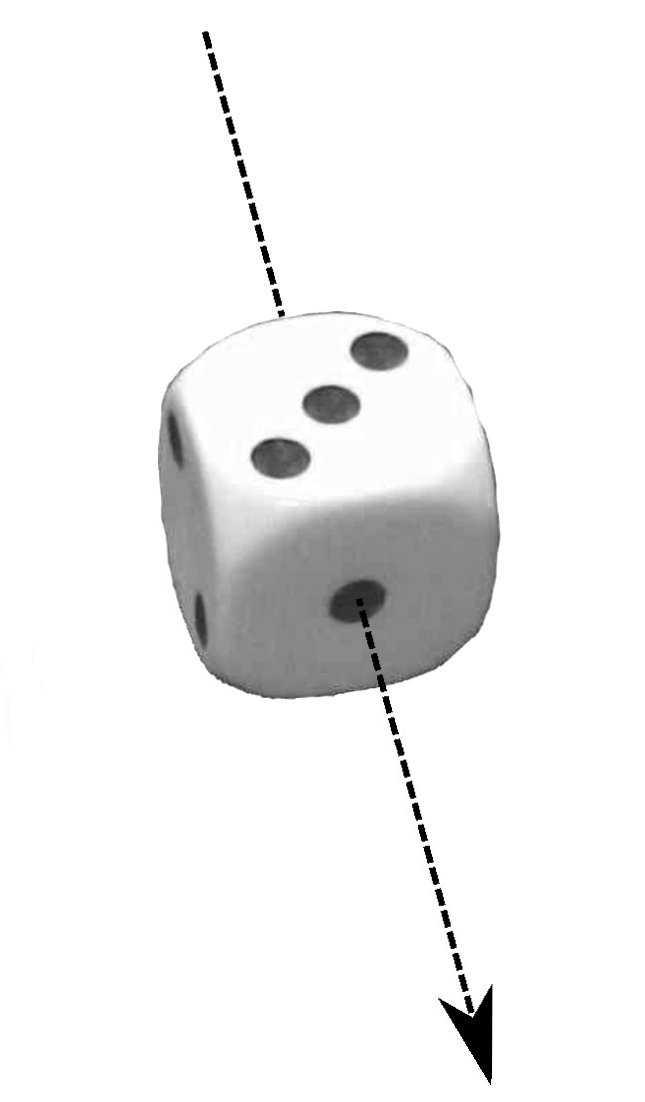
\includegraphics[width=2cm]{pics/deviation_dice.png}
\caption{Representing the Direction Dice with a standard D6.}
\label{figure/deviation_dice}
\end{figure}
